\chapter{Literature Review}

\nomenclature{CNN}{Convolutional Neural Network}
\nomenclature{LSTM}{Long Short Term Memory}
\nomenclature{BiLSTM}{Bidirectional Long Short Term Memory}
\nomenclature{RWF}{Real-World Fights}
\nomenclature{RNN}{Recurrant Neural Network}
\nomenclature{ResNet}{Residual Network}
\nomenclature{ConvLSTM}{Convolutional Long Short Term Memory}
\nomenclature{UCF}{University of Central Florida}
\nomenclature{AUC}{Area Under Curve}
\nomenclature{SPIL}{Skeleton Points Interaction Learning}
\nomenclature{SepConvLSTM}{Separable Convolutional LSTM}
\nomenclature{SSHA}{Semi-Supervised Hard Attention}
\nomenclature{RGB}{Red Green Blue}
\nomenclature{3D}{3-dimensional}
\nomenclature{LaM-2SRN}{Local Features Enhanced and Moving target detected 2Stream-ResNet}
\nomenclature{CAM}{Class Activation Map}
\nomenclature{C3D}{Convolutional 3D}

\setcounter{equation}{0}
\setlength{\parskip}{3ex}

\section{Introduction}

\vspace{-5mm}

\noindent The literature survey explores the domain of violence detection and crowd management in surveillance videos, focusing on the application of deep learning techniques. These approaches are vital for ensuring public safety and security in various contexts, ranging from public spaces to high-security environments. By leveraging advanced algorithms and deep learning models, researchers aim to develop systems capable of automatically identifying violent incidents and analyzing crowd behavior in real time.

\noindent M. Shubber et. al.'s study on integrating machine learning and deep learning approaches \cite{violence_review} has yielded promising results in video violence identification. CNN was a reliable technique for extracting features from video frames, enabling accurate detection of violent behavior. Additionally, LSTM networks have been effective in capturing temporal dependencies in video sequences, overcoming issues like vanishing gradients, and leveraging time dimension information for improved analysis. However, a notable drawback of both CNNs and LSTMs is their reliance on supervised learning, where a large number of labeled training samples are required for training. Moreover, the computational demands of training these models can be substantial, requiring expensive hardware resources, which presents a practical challenge for widespread implementation in surveillance systems.

\clearpage

\noindent S. Lomlen's views on the exponential growth of AI \cite{ai_national_security} also present unprecedented opportunities for enhancing national security and safety across various domains. AI technologies offer the potential to revolutionize defense and military operations by enabling advanced threat detection, decision support systems, and autonomous capabilities. However, the integration of AI in high-stakes contexts like defense and military operations also brings forth significant challenges. One of the primary concerns is the lack of robustness, dependability, and safety of implementing AI methods in critical scenarios, where system failures or inaccuracies could have severe consequences. Additionally, ethical concerns arise regarding the decision-making capability of AI systems, especially in situations involving human lives and complex geopolitical dynamics. Addressing these challenges is crucial to harnessing the full potential of AI while ensuring the safety, security, and ethical integrity of its applications in national security contexts.

\section{Existing Solutions}

\noindent H.Gupta and Syed T.Ali's research \cite{lstm&bilstm} employs LSTM and Bidirectional LSTM (BiLSTM) models for violence detection. LSTM and BiLSTM are recurrent neural network architectures known for their ability to capture temporal dependencies in sequential data, making them well-suited for analyzing video sequences. These models are trained on annotated surveillance video data to learn patterns indicative of violent behavior. However, despite their effectiveness, these models come with computational challenges and may require significant resources for training and inference.

\noindent K.Aarthy and A.Alice Nithya's approach \cite{hockey} focuses on violence detection using the Hockey dataset. To reduce computational costs, the study employs keyframe extraction, a technique that selects representative frames from video sequences. While this approach helps mitigate computational demands, it may struggle with generalization to new and diverse datasets. Additionally, suboptimal hyperparameter tuning could lead to decreased model performance, highlighting the importance of robust experimental design and optimization techniques.

\noindent M.Cheng et. al. have created and introduced the RWF-2000 dataset for violence detection \cite{ourdataset}. This dataset consists of 2,000 video clips captured from real-world scenarios, providing researchers with a valuable resource for training and evaluating violence detection algorithms. Figure \ref{fig:rwfpipeline} shows the data collection pipeline of the RWF-2000 dataset. The Flow Gated Network, a unique architecture designed for this task, incorporates a self-learning pooling mechanism to enhance feature extraction from video data. However, the reliance on large amounts of labeled data for training poses a challenge, as annotating video content, especially violence-related material, can be labor-intensive and sensitive. \\
%\ref{fig:rwfpipeline}
\begin{figure}[htbp!]
    \centering
    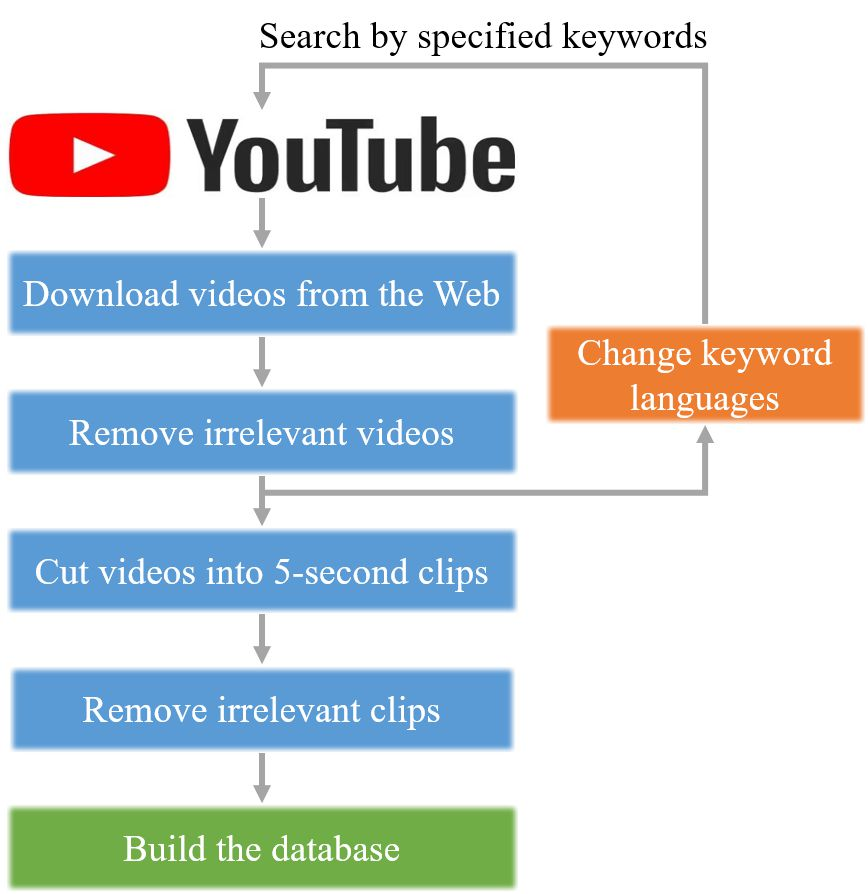
\includegraphics[width=0.7\linewidth]{Images/rwf_pipeline.jpg}
    \caption{RWF-2000 Data Collection Pipeline}
    \label{fig:rwfpipeline}
\end{figure}

\vspace{-5mm}

\noindent In the domain of crowd management, Y.Zuo et. al. have introduced the V3Trans-Crowd framework \cite{vvit}, which leverages a 3D visual transformer for analyzing crowd behavior in public spaces. This novel approach offers improved accuracy compared to existing methods, as demonstrated on the Crowd-11 dataset. 

\clearpage

\noindent However, accurately classifying complex crowd behaviors remains a challenge, highlighting the need for further research into nuanced behavior recognition and classification techniques.

\noindent S.Vosta and K-C.Yow proposes a CNN-RNN structure for violence detection in surveillance camera feeds \cite{cnn-rnn}, combining Residual Network50 (ResNet) for feature extraction and ConvLSTM for anomaly detection. Unlike prior works on hand-crafted datasets, this study uses real-time surveillance feeds with diverse scenarios. It achieves promising results on the University of Central Florida (UCF) Crime dataset, surpassing models like Convolutional 3D (C3D) in Area under Curve (AUC). This research advances automated surveillance for enhanced security monitoring in public and private spaces.

\noindent A.Chauhan et. al. presents an overview of recent advancements in violence detection utilizing deep learning methodologies \cite{lhogf-deeplearn}. Studies such as Tiwari et al. \cite{hyb-cnn-lstm}, Bagga et al. \cite{mobnetv2-inceptionv3}, and Chauhan and Gupta \cite{lhogf-deeplearn} explore the application of CNN and hybrid models like the LHOGF algorithm combined with deep learning for real-time violence detection from Closed-Circuit Television (CCTV) footage. Despite achieving promising results, challenges such as processing delays in object detection remain, suggesting the need for further refinement and optimization of these models to enhance their real-time performance and accuracy.

\noindent R.G.Tiwari et. al. presents a novel approach for automated violence detection and classification in surveillance systems through a hybrid CNN-LSTM model \cite{hyb-cnn-lstm}. By leveraging the strengths of CNN and LSTM networks, the proposed model achieves exceptional accuracy of 98.63\%, surpassing both conventional machine learning methods and state-of-the-art deep learning systems. Through meticulous data collection and preprocessing techniques, the model was trained on a dataset comprising 11,043 images. The study underscores the effectiveness of the hybrid model in enhancing detection and classification skills for violent and nonviolent images in surveillance footage. Further research avenues include exploring additional hybrid architectures, optimizing hyperparameters, and expanding the model's capabilities to recognize a broader range of violent actions.

\clearpage

\noindent Y.Lyu and Y.Yang have presented a novel violence detection algorithm based on local spatio-temporal features and optical flow \cite{Harris3d-spatio-temporal}. Unlike existing methods, this algorithm combines a physical contact detection algorithm with Harris 3D spatio-temporal interest point detection and optical flow to overcome computational challenges. By analyzing motion coefficients, it accurately identifies aggressive actions, distinguishing them from non-violent behaviors. Experimental results demonstrate the algorithm's effectiveness in real-time violence detection, particularly in scenarios involving multiple individuals.

\noindent Deepak K. et. al. presents a novel approach for violence detection using spatio-temporal autocorrelation of gradient-based features \cite{svm-knn-stacog}. The study addresses the challenge of recognizing violent activities in crowded scenes, where traditional methods like trajectory analysis fail due to complex motion and occlusions. By focusing on simpler models, the proposed method, effectively extracts features and reduces computational complexity.

\noindent P.Sernani et. al. has introduced three deep learning-based models for automatic violence detection in videos and evaluate them on the AIRTLab dataset \cite{airtlab}, specifically designed to challenge robustness against false positives. The schematic of all three models used on this dataset is given in Figure \ref{fig:airtlab}. The study emphasizes the importance of addressing misclassifications of friendly behaviors as violent actions. Transfer learning-based models exhibit stable accuracy across datasets, outperforming traditional approaches tested on benchmark datasets. Furthermore, 3D CNN-based models show superiority over 2D CNNs in processing spatio-temporal features, highlighting the potential of 3D architectures for violence detection. Despite challenges posed by imbalanced data, the AIRTLab dataset effectively tests the models' robustness. Future research aims to deepen comparisons between transfer learning and training from scratch approaches on various datasets. The paper underscores the significance of ongoing exploration in deep learning techniques for violence detection in surveillance videos.

\noindent Y. Su et. al. has introduced a new method for recognizing violent behavior by learning contextual relationships between related people from human skeleton points. The proposed Skeleton Points Interaction Learning (SPIL) module \cite{SPIL} aims to focus on the most relevant parts of skeleton points based on their features and position information. 

\clearpage

\begin{figure}[!htbp]
\centering
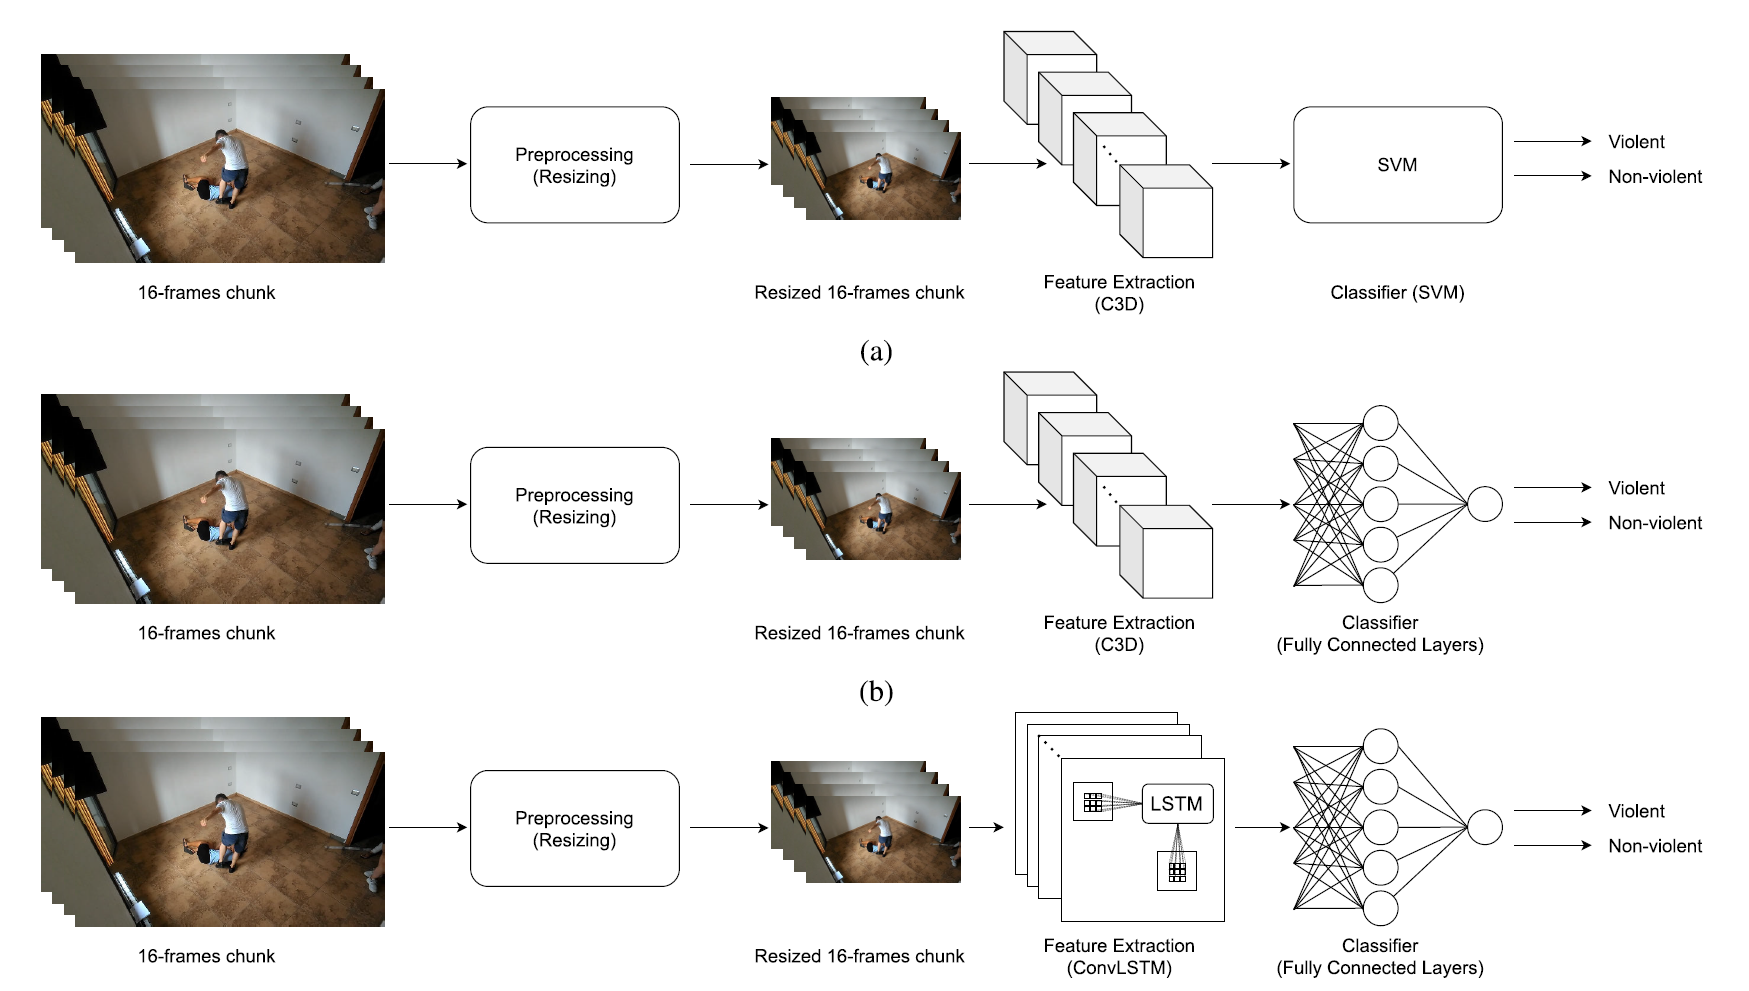
\includegraphics[width=1\linewidth]{Images/airtlab.png}
\caption{Schematic of the Three Models used on AIRTLab Dataset}
%\renewcommand{\label}[1]{}
\label{fig:airtlab}
\end{figure}

\noindent Experimental results show that this model outperforms existing networks and achieves new state-of-the-art performance on video violence datasets. It achieves an accuracy of 89.3\% on the RWF-2000 dataset and 95.5\% on the Hockey dataset and Crowd Violence dataset.

\noindent Z. Islam et. al proposes a deep learning architecture that leverages innovative techniques to automatically detect violence from surveillance footage. The approach combines background suppressed frames and the difference of adjacent frames to highlight moving objects and capture motion, ultimately producing discriminative features for violence detection \cite{SepConvLSTM}. The proposed two-stream deep learning architecture leverages Separable Convolutional LSTM (SepConvLSTM) and pre-trained MobileNet for violence detection to effectively capture spatio-temporal features, distinguish between violent and non-violent actions and achieve state-of-the-art performance on benchmark datasets. \\ The schematic diagram of the proposed pipeline is shown in Figure \ref{fig:sepconvlstm}.
%\ref{fig:sepconvlstm}
\begin{figure}[htbp!]
    \centering
    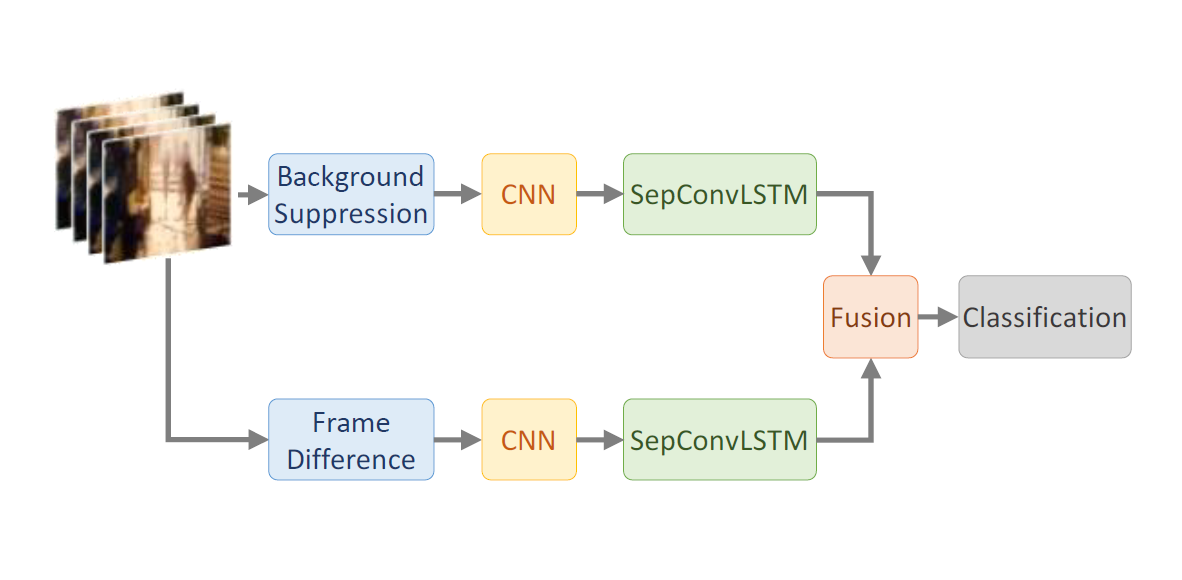
\includegraphics[width=1\linewidth]{Images/sepconv.png}
    \caption{Schematic Diagram of SepConvLSTM Pipeline}
    %\renewcommand{\label}[1]{}
    \label{fig:sepconvlstm}
\end{figure}

\noindent G. Garcia-Cobo et. al. have introduced a novel deep learning architecture that accurately detects violent crimes by focusing on human skeletons and change detection in surveillance footage \cite{HumanSkeleton_ConvLSTM}. By combining these key elements, the proposed method offers a promising solution for real-time crime detection. The model uses human pose extractors to capture spatial relationships in videos, incorporates change detection for identifying sudden movements, and combines these features using addition instead of multiplication. It also utilizes ConvLSTM for efficient processing of spatial and temporal information, enhancing violence detection accuracy.

\noindent H. Mohammadi et. al. discuss SSHA (Semi-Supervised Hard Attention) \cite{SSHM}, a novel deep reinforcement learning model for video violence detection and localization. It addresses the need for scalable AI solutions in video surveillance by leveraging hard attention mechanisms to focus on relevant regions in video frames without relying on computationally expensive auxiliary features like optical flow or pose estimation. SSHA utilizes semi-supervised reinforcement learning, eliminating the need for localization annotations \\ during training, and incorporates a pre-trained I3D backbone network to exploit temporal information. Experimental results demonstrate SSHA's state-of-the-art performance on multiple datasets, achieving accuracy rates of 90.4\% on RWF and 98.7\% on Hockey datasets with the RGB-only architecture, surpassing existing methods and showcasing the effectiveness of the hard attention approach.

\noindent R. Hachiuma et. al. proposes a novel deep neural network architecture called Structured Keypoint Pooling \cite{structured_kepoint_pooling} to address limitations in conventional skeleton-based action recognition. With state-of-the-art accuracy and impressive speed on a single GPU, the proposed framework offers a solution to skeleton detection and tracking errors, poor variety of targeted actions, and person-wise and frame-wise action recognition challenges. The framework treats time-series key points as a 3D point cloud, allowing for sparse feature aggregation and mitigating errors associated with skeleton detection and tracking. This approach enables a broader range of actions to be targeted, including interactions with nonhuman objects, without relying on tracking algorithms. By leveraging this tracking-free architecture and sparse feature aggregation, the framework demonstrates improved performance in action recognition tasks compared to conventional methods, highlighting the effectiveness of the point cloud deep-learning paradigm.

\noindent Y. Qiao et. al. focuses on LaM-2SRN \cite{LaM-2SRN}, a method designed to enhance local features and detect moving objects for action recognition. This paper explores a novel approach using a 3D CNN model to extract attention-enhanced spatiotemporal features for improved human action recognition. The LaM-2SRN model utilizes the traditional CAM (Class Activation Map) algorithm for visual attention in human action recognition by employing it as a target detection method to obtain optical flow information specifically from the human region. This helps in eliminating the influence of irrelevant optical flow information, such as background clutter, which can interfere with accurate action recognition. By focusing on the human body area using the CAM algorithm, the model can extract optical flow information relevant to the actions being performed, enhancing the discriminative features for better recognition accuracy. The input frames extraction network used in this research work and some examples of CAM-images, BE-images, and AE-images generated through the work is shown in Figure \ref{LaM:2SRN}

\begin{figure}[h!]
\centering
\subfloat[The Input Frames Extraction Network] {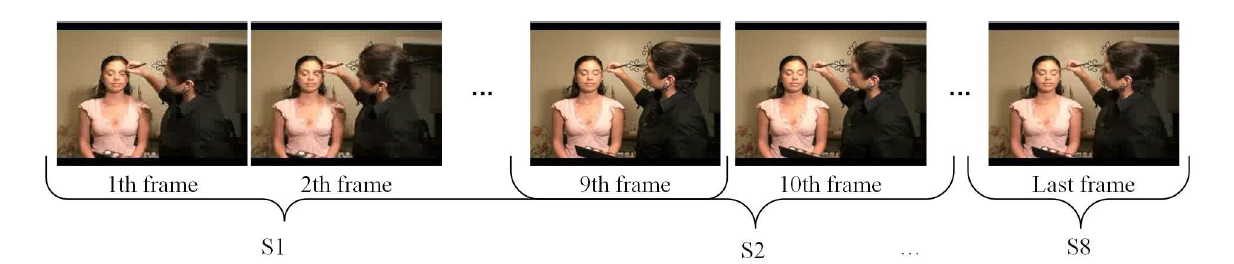
\includegraphics[width=1.05\textwidth]
{Images/lam2 1.png}}
\hfill
\subfloat[Examples of CAM-images, BE-images and AE-images] {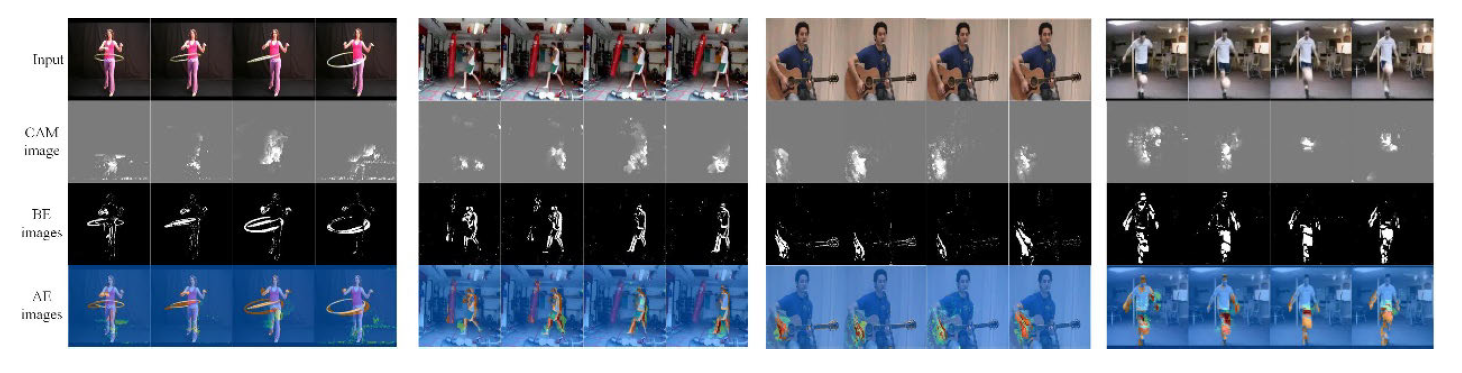
\includegraphics[width=1.05\textwidth]
{Images/lam2 2.png}}
\caption{Activation and Saliency Maps}
    \label{LaM:2SRN}
\end{figure}

%\newpage <use \clearpage>

\section{Summary}

\noindent Various studies and research have led to the domain of violence detection in surveillance videos using machine learning and deep learning techniques. These approaches make use of advanced methodologies such as CNN, LSTM networks, and hybrid models to effectively extract spatio-temporal features from video frames. CNNs excel at feature extraction from visual data, enabling accurate identification of violent behavior patterns. Meanwhile, LSTM networks specialize in capturing temporal dependencies within sequential data, making them ideal for analyzing video sequences. Hybrid models combine the strengths of both CNNs and LSTMs, offering enhanced performance in violence detection tasks. Despite their success, these techniques encounter challenges, and addressing these challenges is crucial for refining existing models and exploring innovative approaches to further improve the accuracy and efficiency of violence detection in surveillance systems.

\clearpage

\noindent Deploying state-of-the-art violence detection models on edge devices like surveillance cameras faces several challenges as discussed before. Firstly, these models tend to be large, exceeding the storage and processing capacities of such devices. This limitation affects their feasibility for deployment in resource-constrained environments. Moreover, the extensive training time and high hardware demands further worsen this issue, making it challenging to train and run these models efficiently. Additionally, concerns about overfitting and the pursuit of enhanced classification accuracy contribute to increased computational requirements during both the training and inference phases. Consequently, implementing these models on edge devices becomes problematic due to the devices' limited computational resources and storage capacity, posing significant obstacles to accommodating the model parameters effectively.

\noindent Overall, the conclusion is that various machine learning and deep learning techniques can be employed for violence detection in surveillance videos, leveraging spatio-temporal features extracted from video frames. However, doing so in edge devices like surveillance cameras is challenging, thus limiting their feasibility and effectiveness in resource-constrained environments. To overcome these issues, there is a need to develop a shallow network with additional mechanisms for classification. For this, the team created a model less prone to overfitting while ensuring it fits within the memory constraints of edge devices like surveillance cameras. By optimizing the architecture to train efficiently on hardware with reasonable specifications, such a model can achieve effective violence detection while overcoming the challenges associated with memory limitations and hardware requirements.

\lfoot{\textit{Departmant of Artificial Intelligence and Data Science, SJCET Palai}}
\renewcommand{\footrulewidth}{0.4pt}